%! TEX root = main.tex
\documentclass[main.tex]{subfiles}
\begin{document}
\section{Laser-Metal-Deposition}
Laser-Metal-Deposition (LMD), auch bekannt als Directed-Energy-Deposition, ist ein weiteres Metall-3D-Druck-Verfahren. LMD ist ein Überbegriff für Schweißraupen-basiertes Additive Manufacturing, da viele weitere Verfahren existieren wie Electron-Beam-Melting.
\begin{figure}[h!]
	\begin{center}

		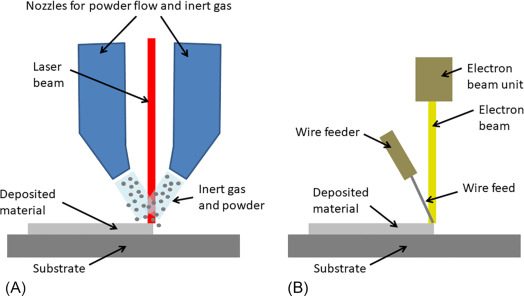
\includegraphics{lmd_1}
\ccaption{Aufbau zweier LMD-Konzepte}{\url{https://ars.els-cdn.com/content/image/3-s2.0-B9780081026632000022-f02-04-9780081026632.jpg}}
\label{img:lmd_1}	
	\end{center}
\end{figure}
Abb. \ref{img:lmd_1} zeigt die beiden wichtigisten Verfahren dieser Übergruppe: (a) Laser-DED \& (b) Electron-Beam-DED.
Bei (a) wird das Druckmaterial durch die Düse eingeschossen in den Laser, welcher es dann auf das bereits daliegende Material aufträgt. 
Dagegen wird bei (b) mithilfe eines Elektronen-Strahls ein Draht aufgeschmolzen und aufgetragen. \parencite{ALL3D_1}

\subsection{Arten von LMD-Maschinen}
\subsubsection{3-Dimensionale Maschinen}

\end{document}
